d\ocumentclass[onecolumn,preprint,superscriptaddress,nofootinbib,notitlepage,10pt,linenumbers]{revtex4-1}

\usepackage[perpage]{footmisc} %the perpage package
\usepackage{epstopdf}
\usepackage{epsfig}
\usepackage{color}
%\usepackage[nativepdf]{hyperref}
\usepackage{mathbbol}
%\usepackage{bookmark}
\usepackage{mathtools}
\usepackage{bbold}
\usepackage{amsmath}
\usepackage{amssymb}
\usepackage{slashed}
\usepackage{nicefrac}
\usepackage{tikz-feynman}
\usepackage{cjhebrew}

\setlength{\topmargin}{-1.0cm}
\setlength{\headheight}{0.1cm} \setlength{\footskip}{1.cm}
\setlength{\headsep}{.1cm}
\setlength{\textheight}{.8\paperheight}
\setlength{\textwidth}{.8\paperwidth}
\setlength{\oddsidemargin}{-.5cm}
\setlength{\evensidemargin}{0.0cm}
\setlength{\marginparwidth}{0.0cm}
\setlength{\marginparsep}{0.0cm}

\definecolor{blue}{HTML}{4169E1}
\definecolor{red}{HTML}{DC143C}
\definecolor{green}{HTML}{2E8B57}
\definecolor{black}{HTML}{000000}
\definecolor{g1}{HTML}{A9A9A9}
\definecolor{g2}{HTML}{696969}
\definecolor{g3}{HTML}{7F7F7F}
\definecolor{g4}{HTML}{D3D3D3}

\newcommand{\caf}{\text{\cjRL{b}}}
\newcommand{\he}{${}^4$He}
\newcommand{\hes}{${}^3$He}
\newcommand{\tr}{${}^3$H}
\newcommand{\ls}{\ve{L}\cdot\ve{S}}
\newcommand{\eps}{\epsilon}
\newcommand{\as}{a_s}
\newcommand{\at}{a_t}
\newcommand{\ecm}{E_\textrm{\small c.m.}}
\newcommand{\dq}{\mbox{d\hspace{-.55em}$^-$}}
\newcommand{\mpis}{$m_\pi=137~${\small MeV}}
\newcommand{\mpim}{$m_\pi=450~${\small MeV}}
\newcommand{\mpil}{$m_\pi=806~${\small MeV}}
\newcommand{\muh}{\mu_{^3\text{\scriptsize He}}}
\newcommand{\mut}{\mu_{^3\text{\scriptsize H}}}
\newcommand{\mud}{\mu_\text{\scriptsize D}}
\newcommand{\pode}{\beta_{\text{\scriptsize D},\pm1}}
\newcommand{\poh}{\beta_{^3\text{\scriptsize He}}}
\newcommand{\pot}{\beta_{^3\text{\scriptsize H}}}
\newcommand{\com}[1]{{\scriptsize \sffamily \bfseries \color{red}{#1}}}
\newcommand{\eg}{\textit{e.g.}\;}
\newcommand{\ie}{\textit{i.e.}\;}
\newcommand{\cf}{\textit{c.f.}\;}
\newcommand{\be}{\begin{equation}}
\newcommand{\ee}{\end{equation}}
\newcommand{\la}{\label}
\newcommand{\ber}{\begin{eqnarray}}
\newcommand{\eer}{\end{eqnarray}}
\newcommand{\nn}{\nonumber}
\newcommand{\half}{\frac{1}{2}}
\newcommand{\thalf}{\nicefrac[]{3}{2}}
\newcommand{\bs}[1]{\ensuremath{\boldsymbol{#1}}}
\newcommand{\bea}{\begin{eqnarray}}
\newcommand{\eea}{\end{eqnarray}}
\newcommand{\beq}{\begin{align}}
\newcommand{\eeq}{\end{align}}
\newcommand{\bk}{\bs k}
\newcommand{\bt}{B_{^{3}\text{H}}}
\newcommand{\bh}{B_{^{3}\text{He}}}
\newcommand{\bd}{B_\text{D}}
\newcommand{\ba}{B_\alpha}
\newcommand{\rgm}{$\mathbb{R}$GM}
\newcommand{\ev}[1] {|\bra #1  \ket |^2}
\newcommand{\lam}[1]{$\Lambda=#1~$fm$^{-1}$}
\newcommand{\parg}[1] {\paragraph*{-\,\textit{#1}\,-}}
\newcommand{\nopi}{\pi\hspace{-6pt}/}
\newcommand{\ve}[1]{\ensuremath{\boldsymbol{#1}}}
\newcommand{\xvec}{\bs{x}}
\newcommand{\rvec}{\bs{r}}
\newcommand{\sgve}{\ensuremath{\boldsymbol{\sigma}}}
\newcommand{\tave}{\ensuremath{\boldsymbol{\tau}}}
\newcommand{\na}{\nabla}
\newcommand{\bra}{\langle}
\newcommand{\ket}{\rangle}
\newcommand{\tx}{\tilde{x}}
\newcommand{\eftnopi}{\mbox{EFT($\slashed{\pi}$)}}
\newcommand{\threej}[6]{\ensuremath{\begin{pmatrix}#1 & #2 & #3\\#4&#5&#6 \end{pmatrix}}}


\DefineFNsymbols*{lamportnostar}[math]{\dagger\ddagger\S\P\|{\dagger\dagger}{\ddagger\ddagger}}
\setfnsymbol{lamportnostar}
\renewcommand\thefootnote{\fnsymbol{footnote}}
\let\endtitlepage\relax

\begin{document}

\title{Lorentz and Siegert offer Compton their assistance.}
\author{Jean Luc Picard}
\email{jeanluc@1701.ncc}
\affiliation{Starfleet Academy, Fort Baker, San Francisco, Earth}
\date{\today}

\begin{abstract}
We study (elastic) Compton scattering off nuclei as a function of the
nucleon number. We consider processes with an initial state comprised of
photons, pions, protons, and neutrons at energies which are insufficient to
create particles that are not composites of these basic degrees of freedom.
The appropriate theory for amplitudes at momentum scales of the order of the pion mass
is constrained by Galilean, chiral, and $U(1)$-gauge symmetries.
The systematic ordering of the interactions thence admissible, allows us to
resolve the various correlations between observables in systems of different
size, kinematics, level of excitation, {\it etc.}. Thereby, we investigate to what
extent properties of large systems can be understood as consequences of the
two- and three-body interaction, but we also address the practical problem, \eg,
to assess the induced uncertainty in a few-body observable due to that in a
one-body quantity -- {\it To what extent does our poor knowledge about the neutron
polarizability affect predictions of deuteron and helium properties?}

An intriguing problem in its own right is the correct application of the
coupling of the two photons to the hadrons and the meson as specified and well
understood in {\it chiral perturbation theory} -- a relativistic quantum field theory --
in a solution of the non-relativistic few-nucleon problem.
\end{abstract}

%\maketitle

%\section{Schr\"odinger and fields}
%\la{sec:schroed-fields}

\section{A tale of two methods to scatter photons of a deuteron}
\la{sec:benchmark}

Ref.~\cite{Bampa:2011fq} does not explicitly calculate scattering amplitudes -- transition probabilities
between states with one deuteron and one photon in the initial and final states as parametrized
in Eq.~(27) and Fig.~(2) of Ref.~\cite{Bampa:2011fq} -- which are output of calculations
by Hildebrandt~\cite{Hildebrandt:2005ix} who (I am not sure this is true) was the first to resolve
the problem to consider the interacting propagation of the two deuteron-comprising nucleons between
the absorption and creation of the photons in the framework of chiral perturbation theory.
The latter method employs Siegert's theorem -- the approximation of the photon field 
$\ve{e}_\lambda~e^{i\ve{k}\cdot\ve{r}}\approx\ve{\nabla}S(\ve{r})$, \ie, 
as a pure nabla field in order to utilize the conservation of the nuclear current -- to facilitate
the calculation of the amplitude which can alternatively be obtained with the {\it Lorentz Integral
Transform Method}~\cite{0954-3899-34-12-R02}. The latter's application to larger nuclei is, barring
potentially prohibitive numerical complications, viable. To asses its practicality for {\it us},
we reconstruct the amplitude from polarizabilities\footnote{If not stated differently, we use conventions
and notation consistent with Ref.~\cite{Bampa:2011fq}.} via

\begin{align}
T_{\lambda^\prime\lambda}^{fi}(\ve{k}^\prime,\ve{k})=&(-)^{1+\lambda^\prime+I_f-M_i}
\sum_{L^{(\prime)},M^{(\prime)} \atop J}(-)^{L+L^\prime}(2J+1)\threej{I_f}{J}{I_i}{-M_f}{m}{M_i}\threej{L}{L^\prime}{J}{M}{M^\prime}{-m}\nonumber\\
&\underbrace{P_{if,J}^{LL^\prime\lambda\lambda^\prime}(k^\prime,k)}_{=\atop\sum\limits_{\nu,\nu^\prime}{\lambda^\prime}^{\nu^\prime}\lambda^\nu P_{if,J}(M^{\nu^\prime}L^\prime,M^\nu L,k^\prime,k)}
D_{M,\lambda}^L(\ve{k}\to\ve{e}_z)D_{M^\prime,-\lambda^\prime}^{L^\prime}(\ve{k}^\prime\to\ve{e}_z)\nonumber
%
\intertext{with the dipole approx. as used in Ref.~\cite{Bampa:2011fq}, \ie, electric ($\nu^{(\prime)}=0$) $\Rightarrow L^{(\prime)}=1$ transitions, $k=k^\prime$ in c.m. system, and the total spin of the deuteron
$I_{i/f}=1$ and associated $z$-projections $M_{i/f}$, this reads}
%
=&(-)^{\lambda^\prime-M_i}\sum_{M^{(\prime)},J}(2J+1)\threej{1}{J}{1}{-M_f}{m}{M_i}\threej{1}{1}{J}{M}{M^\prime}{-m}P_{if,J}(E1,k)
D_{M,\lambda}^1(\ve{k}\to\ve{e}_z)D_{M^\prime,-\lambda^\prime}^1(\ve{k}^\prime\to\ve{e}_z)\;\;\;.\nonumber
%
\intertext{The rotation matrices align the respective $\ve{k}$ vector with {\emph the} quantization axis, which is $\ve{e}_z$, here.
It is common to represent the effect of the two photons on the nucleus in an angular-momentum basis. 
First, each photon field is multipole expanded seperately, before the various terms of the product of both expansions
are combined to form spherical tensor operators of rank \mbox{$|L-L^\prime|\leq J\leq|L+L^\prime|$}. These may induce a change of
angular momentum -- {\color{gray} In general, the photon can induce spin- and orbital-angular-momentum transitions of arbitrary magnitude
regardless of its nature as a $S=1$ gauge boson. Only if the interaction between this vector particle and fermions is constrained to
momentum- and spin-vector independent couplings, one can disregard $\Delta S$, while $\Delta L$ might be limited through the multipole 
expansion of $A_\mu$.} --
of the deuteron by $\leq J$. In the considered approximation, $\vert I_i-I_f\vert\in\lbrace 0,1,2\rbrace$. The projection $m$ is completely fixed by $M_{i/f}$, and $M^{(\prime)}$ are the
$z$-projections of the multipole $E1$ components of the photons.}
=&(-)^{\lambda^\prime-M_i}\sum_{M^{\prime},J}(2J+1)\threej{1}{J}{1}{-M_f}{m}{M_i}\threej{1}{1}{J}{M}{M^\prime}{-m}P_{if,J}(E1,k)
~d_{M^\prime,-\lambda^\prime}^{(1)}(-\theta)=T_{\lambda^\prime}^{fi}(k,\theta)
\end{align}
We chose $\ve{k}\parallel\ve{e}_z$. Therefore, there is no need to rotate $\ve{k}$ and $D_{M,\lambda}^1(\alpha,\beta,\gamma)=1$.
Note that in the considered dipole approximation, this implies the \underline{$\lambda$ independence of the amplitude?!}
The scattering angle $\theta$ parameterizes the propagation direction of the outgoing photon, and the scattering plane is then
defined such that a rotation about the $y$-axis of $\ve{k}^\prime$ by $-\theta$ aligns $\ve{k}^\prime$ with $\ve{e}_z$.
$$D_{M^\prime,-\lambda^\prime}^1(\alpha_z=0,\beta_y=-\theta,\gamma_z=0)=d^{(1)}_{M^\prime,-\lambda^\prime}(-\theta)\;\;\;.$$

\begin{figure}
  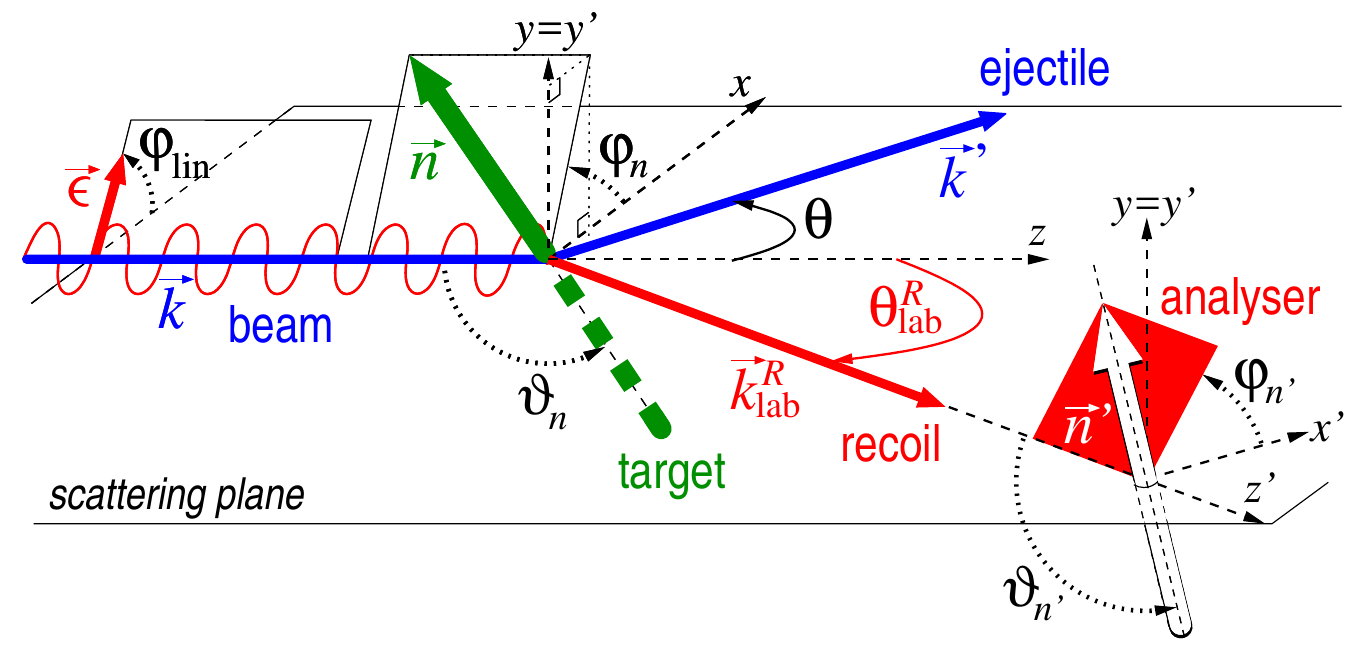
\includegraphics[width=\columnwidth]{kinematics}

  \caption{\label{fig.kinemat} Scattering geometry as taken from Ref.~\cite{Griesshammer:2017txw}.}
\end{figure}


\newpage

\section{formulas and constants}

\begin{alignat}{2}
\text{(Wigner) 3-$j$ symbol:} &\hspace{1cm}& \threej{L}{S}{J}{m_l}{m_s}{-m_j}=&~(-1)^{L-S+m_j}~(2J+1)^{-\frac{1}{2}}~(Lm_l~Sm_s~\vert~LS~Jm_j)\\
\text{Matrix for single-axis rotation:} &\hspace{1cm}&   \mathcal{D}_{m^\prime,m}^{(j)}(0~\beta~0)\equiv&~d_{m^\prime,m}^{(j)}(\beta)\nonumber\\
&\hspace{1cm}& =&\left[\frac{(j+m^\prime)!(j-m^\prime)!}{(j+m)!(j-m)!}\right]^\frac{1}{2}\nonumber\\
&\hspace{1cm}&&~\cdot\sum_\sigma\left(j+m\atop j-m^\prime-\sigma\right)\left(j-m\atop \sigma\right)(-1)^{j-m^\prime-\sigma}\nonumber\\
&\hspace{1cm}&&~\cdot\left(\cos\frac{\beta}{2}\right)^{2\sigma+m+m^\prime}\left(\sin\frac{\beta}{2}\right)^{2j-2\sigma-m-m^\prime}
\end{alignat}

\bibliography{refs}

\end{document}